\documentclass[sigplan, twocolumn]{amsart}
%\usepackage[ruled,vlined,commentsnumbered,titlenotnumbered]{algorithm2e}


\usepackage{enumitem}
\usepackage{subcaption}

\usepackage{tikz,pgfplots}
\usepackage{etoolbox}
%% This makes the colors annoyingly bright, but at least they're easy to distinguish.
\pgfplotsset{
  every  tick/.style={red,}, minor x tick num=1,
  cycle list={teal,every mark/.append style={fill=teal!80!black},mark=*\\%
orange,every mark/.append style={fill=orange!80!black},mark=square*\\%
cyan!60!black,every mark/.append style={fill=cyan!80!black},mark=otimes*\\%
red!70!white,mark=star\\%
lime!80!black,every mark/.append style={fill=lime},mark=diamond*\\%
red,densely dashed,every mark/.append style={solid,fill=red!80!black},mark=*\\%
yellow!60!black,densely dashed,
every mark/.append style={solid,fill=yellow!80!black},mark=square*\\%
black,every mark/.append style={solid,fill=gray},mark=otimes*\\%
blue,densely dashed,mark=star,every mark/.append style=solid\\%
red,densely dashed,every mark/.append style={solid,fill=red!80!black},mark=diamond*\\%
}
}

\def \CILKserialbaseline {4267}
\def \CILKblocksize {64}
\def \CILKnumtrials {1}
\def \CILKinputsize {1073741824}
\def \CILKtable {
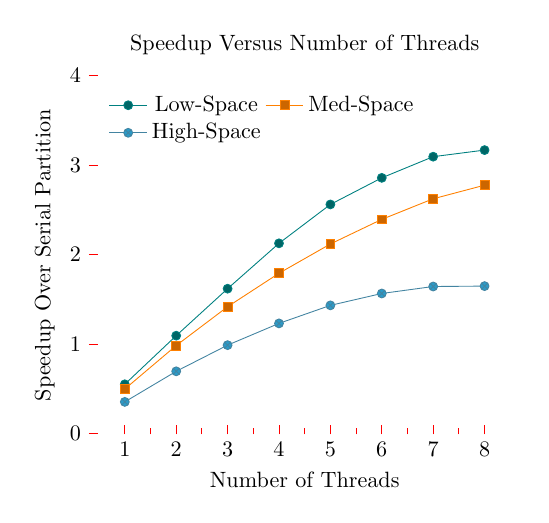
\begin{tikzpicture}[scale = .8]
\begin{axis}[
title={Speedup Versus Number of Threads},
xtick pos=left,
ytick pos=left,
legend style={draw=none},
axis line style = { draw = none },
legend pos= north west,
xtick = data,
xlabel={Number of Threads},
ylabel={Speedup Over Serial Partition},
ymax = 4,
legend columns = 2,
scatter/classes=%
{a={mark=o,draw=blue}}]
%% In-Place
\addplot coordinates {( 1, 0.552935) ( 2, 1.09607) ( 3, 1.6212) ( 4, 2.12818) ( 5, 2.56276) ( 6, 2.85992) ( 7, 3.09652) ( 8, 3.17013) };
%% In-Place Prefix-Sum
\addplot coordinates {( 1, 0.499766) ( 2, 0.985906) ( 3, 1.41949) ( 4, 1.79361) ( 5, 2.12078) ( 6, 2.39585) ( 7, 2.62585) ( 8, 2.77799) };
%% Out-of-Place
\addplot coordinates {( 1, 0.356118) ( 2, 0.697678) ( 3, 0.990253) ( 4, 1.23324) ( 5, 1.43477) ( 6, 1.5676) ( 7, 1.64558) ( 8, 1.65004) };
\legend{Low-Space, Med-Space, High-Space}
\end{axis}
\end{tikzpicture}
}
\def \CILKblocksizetwo {64}
\def \CILKnumtrialstwo {1}
\def \CILKnumcorestwo {8}
\def \CILKinputsizetwo {1073741824}
\def \CILKtabletwo {
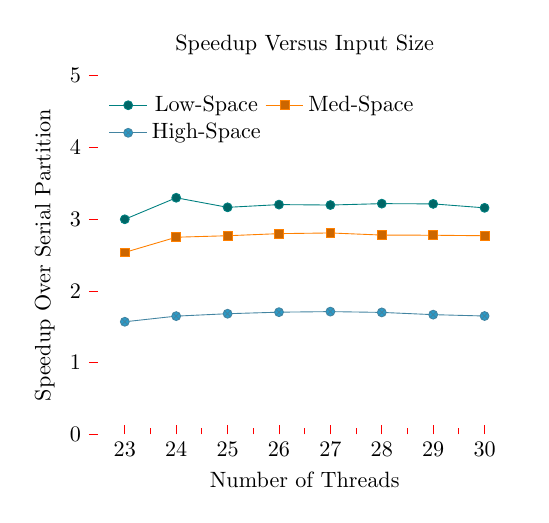
\begin{tikzpicture}[scale = .8]
\begin{axis}[
title={Speedup Versus Input Size},
xtick pos=left,
ytick pos=left,
legend style={draw=none},
axis line style = { draw = none },
legend pos= north west,
xtick = data,
xlabel={Number of Threads},
ylabel={Speedup Over Serial Partition},
ymax = 5,
ymin = 0,
legend columns = 2,
scatter/classes=%
{a={mark=o,draw=blue}}]
%% Serial Baseline
%% baselines in ms: \addplot coordinates {( 23, 33 ) ( 24, 66 ) ( 25, 133 ) ( 26, 266 ) ( 27, 531 ) ( 28, 1062 ) ( 29, 2125 ) ( 30, 4253 ) };
%% In-Place
\addplot coordinates {( 23, 3) ( 24, 3.3) ( 25, 3.16667) ( 26, 3.20482) ( 27, 3.1988) ( 28, 3.21818) ( 29, 3.21483) ( 30, 3.15973) };
%% In-Place Prefix-Sum
\addplot coordinates {( 23, 2.53846) ( 24, 2.75) ( 25, 2.77083) ( 26, 2.8) ( 27, 2.80952) ( 28, 2.7801) ( 29, 2.77778) ( 30, 2.77068) };
%% Out-of-Place
\addplot coordinates {( 23, 1.57143) ( 24, 1.65) ( 25, 1.68354) ( 26, 1.70513) ( 27, 1.7129) ( 28, 1.70192) ( 29, 1.6706) ( 30, 1.65165) };
\legend{Low-Space, Med-Space, High-Space}
\end{axis}
\end{tikzpicture}
}

\def \serialnumtrials {5}
\def \serialblocksize {64}
\def \serialtable {
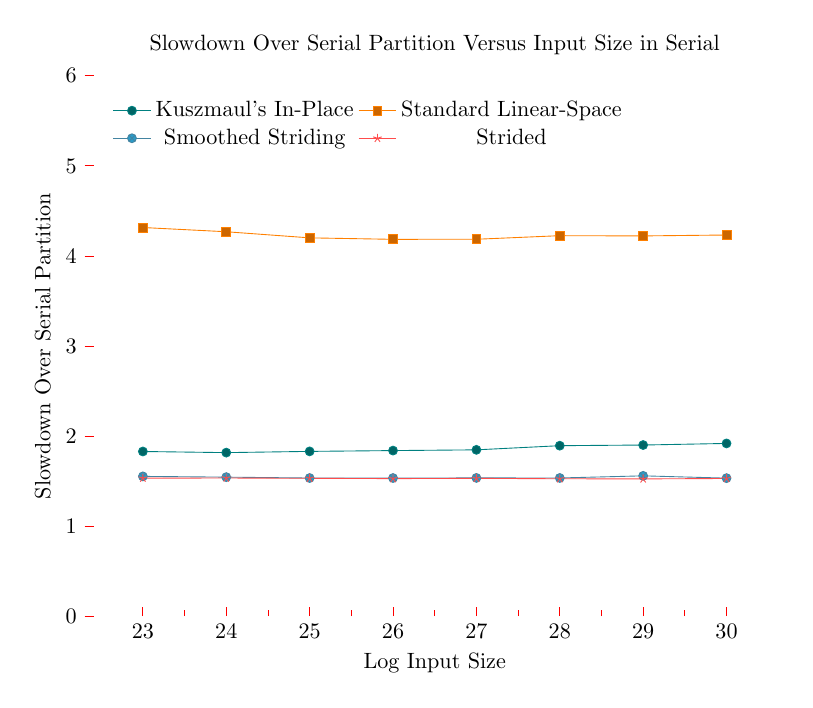
\begin{tikzpicture}[scale = .8]
\begin{axis}[
width = 5 in,
height = 4in,
title={Slowdown Over Serial Partition Versus Input Size in Serial},
xtick pos=left,
ytick pos=left,
ymax = 6,
ymin = 0,
legend style={draw=none},
axis line style = { draw = none },
legend pos= north west,
xtick = data,
xlabel={Log Input Size},
ylabel={Slowdown Over Serial Partition},
legend columns = 2,
scatter/classes=%
{a={mark=o,draw=blue}}]
%% Serial Baseline
%% baselines in ms: \addplot coordinates {( 23, 30.4 ) ( 24, 61 ) ( 25, 122.4 ) ( 26, 244.8 ) ( 27, 489.6 ) ( 28, 979.6 ) ( 29, 1963.4 ) ( 30, 3922.6 ) };
%% In-Place
\addplot coordinates {( 23, 1.82895) ( 24, 1.81639) ( 25, 1.83007) ( 26, 1.83905) ( 27, 1.84722) ( 28, 1.89343) ( 29, 1.90068) ( 30, 1.91837) };
%% In-Place Prefix-Sum
% \addplot coordinates {( 23, 2.75658) ( 24, 2.71803) ( 25, 2.68137) ( 26, 2.67157) ( 27, 2.67443) ( 28, 2.70131) ( 29, 2.70551) ( 30, 2.71713) };
%% Out-of-Place
\addplot coordinates {( 23, 4.31579) ( 24, 4.26885) ( 25, 4.20098) ( 26, 4.18464) ( 27, 4.18546) ( 28, 4.22519) ( 29, 4.22257) ( 30, 4.23265) };
%% %% High-Span
%% \addplot coordinates {( 23, 1.23684) ( 24, 1.23934) ( 25, 1.24346) ( 26, 1.24428) ( 27, 1.24632) ( 28, 1.24602) ( 29, 1.24417) ( 30, 1.2456) };
%% Cache-Friendly
\addplot coordinates {( 23, 1.55263) ( 24, 1.54426) ( 25, 1.53431) ( 26, 1.53431) ( 27, 1.53554) ( 28, 1.53491) ( 29, 1.55852) ( 30, 1.53317) };
%% Strided
\addplot coordinates {( 23, 1.53289) ( 24, 1.53443) ( 25, 1.53105) ( 26, 1.52778) ( 27, 1.53064) ( 28, 1.52613) ( 29, 1.5246) ( 30, 1.52919) };
\legend{Kuszmaul's In-Place, Standard Linear-Space, Smoothed Striding, Strided} % Low-Space, Med-Space, High-Space, Smoothed Striding, Strided
\end{axis}
\end{tikzpicture}
}
%% \def \serialnumtrials {5}
%% \def \serialblocksize {64}
%% \def \serialtable {
%% \begin{tikzpicture}[scale = .8]
%% \begin{axis}[
%% width = 5 in,
%% height = 4in,
%% title={Slowdown Versus Input Size in Serial},
%% xtick pos=left,
%% ytick pos=left,
%% ymax = 5,
%% ymin = 0,
%% legend style={draw=none},
%% axis line style = { draw = none },
%% legend pos= north west,
%% xtick = data,
%% xlabel={Log Input Size},
%% ylabel={Slowdown Over Serial Partition},
%% legend columns = 2,
%% scatter/classes=%
%% {a={mark=o,draw=blue}}]
%% %% Serial Baseline
%% %% baselines in ms: \addplot coordinates {( 23, 30.4 ) ( 24, 61 ) ( 25, 122.4 ) ( 26, 244.8 ) ( 27, 489.6 ) ( 28, 979.6 ) ( 29, 1963.4 ) ( 30, 3922.6 ) };
%% %% In-Place
%% \addplot coordinates {( 23, 1.82895) ( 24, 1.81639) ( 25, 1.83007) ( 26, 1.83905) ( 27, 1.84722) ( 28, 1.89343) ( 29, 1.90068) ( 30, 1.91837) };
%% %% In-Place Prefix-Sum
%% \addplot coordinates {( 23, 2.75658) ( 24, 2.71803) ( 25, 2.68137) ( 26, 2.67157) ( 27, 2.67443) ( 28, 2.70131) ( 29, 2.70551) ( 30, 2.71713) };
%% %% Out-of-Place
%% \addplot coordinates {( 23, 4.31579) ( 24, 4.26885) ( 25, 4.20098) ( 26, 4.18464) ( 27, 4.18546) ( 28, 4.22519) ( 29, 4.22257) ( 30, 4.23265) };
%% %% High-Span
%% \addplot coordinates {( 23, 1.23684) ( 24, 1.23934) ( 25, 1.24346) ( 26, 1.24428) ( 27, 1.24632) ( 28, 1.24602) ( 29, 1.24417) ( 30, 1.2456) };
%% %% Cache-Friendly
%% \addplot coordinates {( 23, 1.55263) ( 24, 1.54426) ( 25, 1.53431) ( 26, 1.53431) ( 27, 1.53554) ( 28, 1.53491) ( 29, 1.55852) ( 30, 1.53317) };
%% %% Strided
%% \addplot coordinates {( 23, 1.53289) ( 24, 1.53443) ( 25, 1.53105) ( 26, 1.52778) ( 27, 1.53064) ( 28, 1.52613) ( 29, 1.5246) ( 30, 1.52919) };
%% \legend{Low-Space, Med-Space, High-Space, Two-Layer, Cache-Friendly, Strided}
%% \end{axis}
%% \end{tikzpicture}
%% }
%% \def \serialnumtrials {1}
%% \def \serialblocksize {64}
%% \def \serialtable {
%% \begin{tikzpicture}[scale = .8]
%% \begin{axis}[
%% title={Slowdown Versus Input Size in Serial},
%% width = 5in, %%!!!!
%% height = 4in,
%% xtick pos=left,
%% ytick pos=left,
%% ymax = 5, %% !!!
%% ymin = 0,
%% legend style={draw=none},
%% axis line style = { draw = none },
%% legend pos= north west,
%% xtick = data,
%% xlabel={Log Input Size},
%% ylabel={Slowdown Over Serial Partition},
%% legend columns = 2,
%% scatter/classes=%
%% {a={mark=o,draw=blue}}]
%% %% Serial Baseline%% baselines in ms: \addplot coordinates {( 23, 30.4 ) ( 24, 60.8 ) ( 25, 121.4 ) ( 26, 243.8 ) ( 27, 487.4 ) ( 28, 975.8 ) ( 29, 1952.2 ) ( 30, 3902 ) };
%% %% In-Place
%% \addplot coordinates {( 23, 1.79605) ( 24, 1.82237) ( 25, 1.84185) ( 26, 1.84249) ( 27, 1.87033) ( 28, 1.90838) ( 29, 1.90687) ( 30, 1.91579) };
%% %% In-Place Prefix-Sum
%% \addplot coordinates {( 23, 2.58553) ( 24, 2.57237) ( 25, 2.57661) ( 26, 2.56932) ( 27, 2.56422) ( 28, 2.59459) ( 29, 2.60834) ( 30, 2.61107) };
%% %% Out-of-Place
%% \addplot coordinates {( 23, 3.98684) ( 24, 3.96711) ( 25, 3.96705) ( 26, 3.96308) ( 27, 3.98195) ( 28, 4.01537) ( 29, 4.03401) ( 30, 4.06079) };
%% %% High-Span
%% \addplot coordinates {( 23, 1.21053) ( 24, 1.23355) ( 25, 1.23558) ( 26, 1.23298) ( 27, 1.23677) ( 28, 1.24124) ( 29, 1.24096) ( 30, 1.23931) };
%% \legend{Low-Space, Med-Space, High-Space, Two-Layer} %% Two-layer instead of high-span everywhere
%% \end{axis}
%% \end{tikzpicture}
%% }
%% %% Speedup on 18 threads in table of size 268435456
%% \def \serialsortspeedup {0.780189}




\usepackage{url}
\usepackage{fullpage}
%\setlength{\oddsidemargin}{0pt}
%\setlength{\evensidemargin}{0pt}
%\setlength{\textwidth}{6.5in}
%\setlength{\topmargin}{0in}
%\setlength{\textheight}{9in}
%\usepackage{refcheck}
%\usepackage{pslatex} % use times roman
\newcommand{\defn}[1]       {{\textit{\textbf{\boldmath #1}}}}
\renewcommand{\paragraph}[1]{\vspace{0.09in}\noindent{\bf \boldmath #1.}} 
\usepackage{amsmath}
\usepackage{algorithm}
\usepackage[noend]{algpseudocode}
\usepackage{amssymb}
\usepackage{amsthm}
\usepackage{color}
\usepackage{tikz}
\usetikzlibrary{arrows,shapes}
\usetikzlibrary{matrix}
\usepackage{array}
\usepackage{xy}
\usepackage{setspace}
\usepackage{multicol}
\usepackage{algorithm}
\usepackage{hyperref}
%%\doublespacing
%\usepackage{natbib}
%% \usepackage{cite}
%% \usepackage[margin=1in,letterpaper]{geometry}
%% \setlength{\topmargin}{0 in}
%% \setlength{\textheight}{9 in}
\usepackage{todonotes}

%% \documentclass[12pt,letterpaper]{amsart}
%% \setlength{\oddsidemargin}{0pt}
%% \setlength{\evensidemargin}{0pt}
%% \setlength{\textwidth}{6.5in}
%%\setlength{\topmargin}{1in}
%% \setlength{\textheight}{9in}
%% %\usepackage{refcheck}
%% \usepackage{pslatex} % use times roman
%% \usepackage{amsmath}
%% \usepackage{amssymb}
%% \usepackage{amsthm}
%% \usepackage{color}
%% \usepackage{array}
%% \usepackage{xy}
%% \usepackage{setspace}

%\usepackage[left=1.5in,right=1.5in, top=1.5in,bottom=1.5in,]{geometry}

\newcommand{\NN}{\mathbb{N}} \newcommand{\ZZ}{\mathbb{Z}}
\newcommand{\range}{\text{ran}}
\newcommand{\poly}{\operatorname{poly}}
\newcommand{\domain}{\text{dom}} \newcommand{\im}{\text{im}}
\newcommand{\sign}{\operatorname{sign}} \newcommand{\si}{\mathbf{S}}
\newcommand{\OR}{\vee} \newcommand{\E}{\mathbb{E}}
\newcommand{\AND}{\wedge} \newcommand{\PP}{\mathcal{P}}
\newcommand{\edit}{\operatorname{ed}}
\newcommand{\dtw}{\operatornamewithlimits{dtw}}
\newcommand{\ed}{\operatorname{ed}}
\newcommand{\ham}{\operatorname{Ham}}
\newcommand{\dist}{\Delta_{\ell_1}}
\newcommand{\argmin}{\operatornamewithlimits{argmin}}
\newcommand{\subproblem}{\operatornamewithlimits{endToMiddle}}
\newcommand{\xrun}{r_x} \newcommand{\yrun}{r_y}
\newcommand{\yrunlength}{l_y} \newcommand{\yprevrunlength}{p_y}
\newcommand{\xrunlength}{l_x} \newcommand{\yoffset}{o_y}
\newcommand{\xoffset}{o_x}
\newcommand{\yrunoffset}{o_x}
\newcommand{\xrunoffset}{o_y}
\newcommand{\tipToMiddle}{\operatorname{SP}}
\newcommand{\rundiff}{d}
\newcommand{\dec}{\operatorname{dec}}



%----------------MACROS---------------%
%% \newtheoremstyle{slanted}% <name>
%% {3pt}% <Space above>
%% {3pt}% <Space below>
%% {\slshape}% <Body font>
%% {}% <Indent amount>
%% {\bfseries}% <Theorem head font>
%% {.}% <Punctuation after theorem head>
%% {.5em}% <Space after theorem heading>
%% {}% <Theorem head spec (can be left empty, meaning `normal')>


\newtheorem{thm}{Theorem}[section]
\newtheorem{lem}[thm]{Lemma}
\newtheorem{prop}[thm]{Proposition}
\newtheorem{clm}[thm]{Claim}
\newtheorem{cor}[thm]{Corollary}
\newtheorem{conj}[thm]{Conjecture}
\theoremstyle{remark}
\newtheorem{rem}[thm]{Remark}
\newtheorem{ex}[thm]{Example}

\newtheorem{theorem}{Theorem}[section]
\newtheorem{definition}[thm]{Definition}
\newtheorem{lemma}[thm]{Lemma}
\newtheorem{proposition}[thm]{Proposition}
\newtheorem{claim}[thm]{Claim}
\newtheorem{corollary}[thm]{Corollary}
\newtheorem{conjecture}[thm]{Conjecture}
\theoremstyle{remark}
\newtheorem{remark}[thm]{Remark}
\newtheorem{example}[thm]{Example}
\newtheorem{observation}[thm]{Observation}

\usepackage{hyperref}
%-----------------Beginning document.
\begin{document}

\title{A Simple In-Place Parallel Partition using Exclusive-Read-and-Write Memory}
\author{William Kuszmaul }
\maketitle


  \begin{abstract}
We present a simple in-place algorithm for parallel partition that has
work $O(n)$ and span $O(\log n \cdot \log \log n)$. The algorithm uses
only exclusive read/write shared variables, and can be implemented
using parallel-for-loops without any additional concurrency
considerations (i.e., the algorithm is in the EREW PRAM model). As an
immediate consequence, we also get a simple in-place quicksort
algorithm with work $O(n \log n)$ and span $O(\log^2 \log \log n)$.

Using our algorithmic techniques, we implement an (almost) in-place
parallel-prefix. In addition to achieving much better memory
utilization, the algorithm achieves a modest speedup over its
out-of-place counterpart.
 \end{abstract}

\section{Introduction}

A \defn{parallel partition} operation rearranges the elements in an
array so that the elements satisfying a particular \defn{pivot
  property} appear first. In addition to playing a central role in
parallel quicksort, the parallel partition operation is used as a
primitive throughout parallel algorithms.\footnote{In several
  well-known textbooks and surveys on parallel algorithms
  \cite{AcarBl16,Blelloch96}, for example, parallel partitions are
  implicitly used extensively to perform what are referred to as
  \emph{filter} operations.}

A parallel algorithm can be measured by its \defn{work}, the time
needed to execute in serial, and its \defn{span}, the time to execute
on infinitely many processors. There is a well-known algorithm for
parallel partition on arrays of size $n$ with work $O(n)$ and span
$O(\log n)$ \cite{Blelloch96,AcarBl16}. Moreover, the algorithm uses
only exclusive read/write shared memory variables (i.e., it is an
\defn{EREW} algorithm). This eliminates the need for concurrency
  mechanisms such as locks, and ensures good behavior even if the time
  to access a location is a function of the number of threads trying
  to access it (or its cache line) concurrently.

The parallel algorithm differs from its serial counterpart in the use
of extra memory, however. Whereas the serial algorithm is typically
implemented in place, the parallel algorithm relies on the use of two
auxiliary arrays of size $n$. To the best of our knowledge, the only
linear-work and $\operatorname{polylog}(n)$-span algorithms for
parallel partition that \emph{are} in-place require the use of atomic
operations (e.g, fetch-and-add)
\cite{HeidelbergerNo90,AxtmannWi17,TsigasZh03}. 

An algorithm's memory efficiency can be critical on large inputs. The
memory consumption of an algorithm determines the largest problem size
that can be executed in memory. Many external memory algorithms (i.e.,
algorithms for problems too large to fit in memory) perform large
subproblems in memory; the size of these subproblems is again
bottlenecked by the algorithm's memory-overhead \cite{Vitter08}. In
multi-user systems, memory efficiency is also important on small
inputs, since processes with larger memory-footprints can hog the
cache, slowing down other processes.

For sorting algorithms, in particular, special attention to memory
efficiency is often given. In the context of parallel algorithms,
however, the most practically efficient algorithms fail to run in
place, at least without the additional use of atomic-fetch-and-add
variables \cite{HeidelbergerNo90, AxtmannWi17, TsigasZh03}, or the
loss of theoretical guarantees on parallelism
\cite{FrancisPa92}. Parallel merge sort \cite{Hagerup89} was made
in-place by Katajainen \cite{Katajainen93}, but has proven too
sophisticated for practical applications. Bitonic sort
\cite{BlellochLe98} is naturally in-place, and can be practical in
certain applications on super computers, but suffers in general from
requiring work $\Theta(n \log^2 n)$ rather than $O(n \log
n)$. Parallel quicksort, on the other hand, despite the many efforts
to optimize it \cite{HeidelbergerNo90, AxtmannWi17, TsigasZh03,
  FrancisPa92, Frias08}, has eluded any in-place EREW algorithms due
to its reliance on parallel partition.


\paragraph{Results}
We present a simple in-place algorithm for parallel partition that has
work $O(n)$ and span $O(\log n \cdot \log \log n)$. The algorithm uses
only exclusive read/write shared variables, and can be implemented
using parallel-for-loops without any additional concurrency
considerations. As an immediate consequence, we also get a simple
in-place quicksort algorithm with work $O(n \log n)$ and span
$O(\log^2 \log \log n)$.

The simplicity of our algorithmic techniques makes them condusive to
practical implementations. We implement and optimize an (almost)
in-place implementation. Because the in-place algorithm eliminates the
use of large auxilary arrays, the algorithm is able to achieve a
significant reduction in cache misses over its out-of-place
counterpart. In addition to significantly reducing the memory
overhead, the space-efficient algorithm is able to achieve a modest
performance improvement, and on a single thread performs within a
factor of two of the in-place serial algorithm.

\section{Preliminaries}\label{secprelim}

We begin by describing the the parallelism and memory model used in
the paper, and by presenting background on parallel partition.

\paragraph{Workflow Model} We consider a language-based model of parallelism in which algorithms may achieve parallelism
through the use of \defn{parallel-for-loops}, though our algorithm
also works in the less restrictive EREW PRAM model
\cite{Blelloch96,AcarBl16}.  A parallel-for-loop is given a range $R
\in \mathbb{N}$, a constant number of arguments $\arg_1, \arg_2,
\ldots, \arg_c$, and a body of code. For each $i \in \{1, \ldots,
R\}$, the loop launches a thread that is given loop-counter $i$ and
local copies of the arguments $\arg_1, \arg_2, \ldots, \arg_c$. The
threads then perform the body of the loop.\footnote{Note that
  parallel-for-loops also implicitly allow for the implementation of
  parallel recursion by placing recursive function calls in the body
  of the parallel-for-loop.}

A parallel algorithm may be run on an arbitrary number $p$ of
processors. The algorithm itself is oblivious to $p$, however, leaving
the assignment of threads to processors up to a scheduler.

The \defn{work} $T_1$ of an algorithm is the time that the algorithm
would require to execute on a single processor. The \defn{span}
$T_\infty$ of an algorithm is the time to execute on infinitely many
processors. The scheduler is assumed to contribute no overhead to the
span. In particular, if the body of a
parallel-for-loop has span $s$, then the full parallel loop has span
$s + O(1)$ \cite{Blelloch96,AcarBl16}.

The work $T_1$ and span $T_\infty$ can be used to quantify the time $T_p$
that an algorithm requires to execute on $p$ processors using a greedy
online scheduler. If the scheduler is assumed to contribute no
overhead, then Brent's Theorem \cite{Brent74} states that for any
$p$,
$$T_1 / p \le T_p \le T_1 / p + T_\infty.$$

The work-stealing algorithms used in the Cilk extension of C/C++ realize
the guarantee offered by Brent's Theorem within a constant factor
\cite{BlumofeJo96,BlumofeLe99}, with the added caveat that parallel
for-loops typically induce an additional additive overhead of $O(\log
R)$.

\paragraph{Memory Model} Memory is \defn{exclusive-read} and \defn{exclusive-write}. That is, no two threads are ever permitted to attempt to read or write to the same variable concurrently. The exclusive-read exclusive-write memory model is sometime referred to as the \defn{EREW model} (see, e.g., \cite{Hagerup89}).

In an \defn{in-place} algorithm, each thread is given $O(\log n)$
memory upon creation that is deallocated when the thread dies. This
memory can be shared with the thread's children. The depth of the
parent-child tree is not permitted to exceed $O(\log n)$.\footnote{The
  algorithm in this paper satisfies a slightly stronger property that
  the total memory being used is never more than $O(\log n) \cdot p$,
  where $p$ is an upper-bound on the number of worker threads.}

\paragraph{The Parallel Partition Problem}
The parallel partition problem takes an input array $A$ of size $n$,
and a \defn{decider function} $\dec$ that determines for each element
$a[i] \in A$ whether or not $A[i]$ is a \defn{predecessor} or a
\defn{successor}. That is, $\dec(A[i]) = 1$ if $A[i]$ is a predecessor,
and $\dec(A[i]) = 0$ if $A[i]$ is a successor. The behavior of the
parallel partition is to reorder the elements in the array $A$ so that
the predecessors appear before the successors.


\paragraph{The (Standard) Linear-Space Parallel Partition} The linear-space implementation of parallel partition consists of two phases \cite{Blelloch96,AcarBl16}:

\noindent\emph{The Parallel-Prefix Phase: }In this phase, the algorithm
constructs an array $B$ whose $i$-th element $B[i] = \sum_{j = 1}^i
\dec(A[i])$ is the number of predecessors in the first $i$ elements of
$A$. The transformation from $A$ to $B$ is called a \defn{parallel
  prefix sum} and can be performed with $O(n)$ work and $O(\log n)$
span using a simple recursive algorithm: (1) First construct an array
$A'$ of size $n / 2$ with $A'[i] = A[2i - 1] + A[2i]$; (2)
Recursively construct a parallel prefix sum $B'$ of $A'$; (3) Build
$B$ by setting each $B[i] = B'[\lfloor i / 2 \rfloor] + A[i]$ for odd
$i$ and $B[i] = A'[i / 2]$ for even $i$. 

\noindent\emph{The Reordering Phase: }In this phase, the algorithm
constructs an output-array $C$ by placing each predecessor $A[i] \in A$
in position $B[i]$ of $C$. If there are $t$ predecessors in $A$, then
the first $t$ elements of $C$ will now contain those $t$ predecessors
in the same order that they appear in $A$. The algorithm then places
each successor $A[i] \in A$ in position $t + i - B[i]$. Since $i - B[i]$
is the number of successors in the first $i$ elements of $A$, this
places the successors in $C$ in the same order that they appear in
$A$. Finally, the algorithm copies $C$ into $A$, completing the
parallel partition.

Both phases can be implemented with $O(n)$ work and $O(\log n)$
span. Like its serial out-of-place counterpart, the algorithm is
stable but not in place. The algorithm uses two auxilary arrays of
size $n$. Kiu, Knowles, and Davis \cite{LiuKn05} were able to reduce
the extra space consumption to $n + p$ under the assumption that the
number of processors $p$ is hard-coded; their algorithm breaks the
array $A$ into $p$ parts and assigns one part to each thread. Reducing
the space below $o(n)$ has remained open until now, even when the
number of threads is fixed.

\section{A Simple In-Place Algorithm}\label{secalg}

In this section, we present a simple in-place algorithm for parallel
partition. 

We assume without loss of generality that the total number of
successors in $A$ exceeds the number of predecessors, since otherwise
their roles can simply be swapped in the algorithm. Further, we assume
for simplicity that the elements of $A$ are distinct; this assumption
is removed at the end of the section.


\paragraph{Algorithm Outline}
We begin by presenting an overview of the key algorithmic ideas needed
to construct an in-place algorithm.

Consider how to remove the auxiliary array $C$ from the Reordering
Phase. If one attempts to simply swap in parallel each predecessor
$A[i]$ with the element in position $j = B[i]$ of $A$, then the swaps
will almost certainly conflict. Indeed, $A[j]$ may also be a
predecessor that needs to be swapped with $A[B[j]]$. Continuing like
this, there may be an arbitrarily long list of dependencies on the
swaps.

To combat this, we begin the algorithm with a Preprocessing Phase in
which $A$ is rearranged so that every prefix is
\defn{successor-heavy}, meaning that for all $t$, the first $t$ elements contain at
least $\frac{t}{4}$ successors. Then we compute the
prefix-sum array $B$, and begin the Reordering Phase. Using the
fact that the prefixes of $A$ are successor-heavy, the reordering can
now be performed in place as follows: (1) We begin by recursively
reordering the prefix $P$ of $A$ consisting of the first $4/5 \cdot n$
elements, so that the predecessors appear before the successors; (2)
Then we simply swap each predecessor $A[i]$ with the corresponding
element $B[A[i]]$. The fact that the prefix $P$ is successor-heavy
ensures that the final $\frac{1}{5} \cdot n$ elements of the reordered
$P$ will consist of successors. This implies that for each of the
swaps between predecessors $A[i]$ and earlier positions $B[A[i]]$, the
latter element will be a successor. In other words, the swaps are now
conflict free.

Next consider how to remove the array $B$ from the Parallel-Prefix
Phase. At face value, this would seem quite difficult since the
reordering phase relies heavily on $B$. Our solution is to
\emph{implicitly} store the value of every $O(\log n)$-th element of
$B$ in the ordering of the elements of $A$. That is, we break $A$ into
blocks of size $O(\log n)$, and use the order of the elements in each
block to encode an entry of $B$. (If the elements are not all
  distinct, then a slightly more sophisticated encoding is necessary.)
Moreover, we modify the algorithm for building $B$ to only construct
every $O(\log n)$-th element and to perform the construction also
using implicitly storing values. The new parallel-prefix sum performs
$O(n / \log n)$ arithmetic operations on values that are implicitly
encoded in blocks; since each such operation requires $O(\log n)$
work, the total work remains linear.

In the remainder of the section, we present the algorithm in detail.
It proceeds in three phases.

\paragraph{A Preprocessing Phase} Recall that for each $t \in 1, \ldots, n$, we call the $t$-prefix $A[1], \ldots, A[t]$ of $A$ successor-heavy if it contains at least $\frac{t}{4}$ successors. The goal of the preprocessing phase is to rearrange $A$ so that every prefix is successor heavy.

We begin with a parallel-for-loop: For each $i = 1, \ldots, \lfloor n
/ 2\rfloor$, if $A[i]$ is a predecessor and $A[n - i + 1]$ is a
successor, then we swap their positions in $A$.

This ensures that at least half the successors in $A$ reside in the
first $\lceil n / 2 \rceil$ positions. Thus the first $\lceil n / 2
\rceil$ positions contain at least $\lceil n / 4\rceil$ successors,
making every $t$-prefix with $t \ge \lceil n / 2 \rceil$
successor-heavy.

Since $\lceil n / 4 \rceil \ge \frac{\lceil n / 2 \rceil}{2}$, the
first $\lceil n / 2 \rceil$ positions of $A$ now contain at least as
many successors as predecessors. Thus we can recursively repeat the
same process on the subarray $[A[1], \ldots, A[\lceil n / 2 \rceil]]$
in order to make each of its prefixes successor-heavy.

Each recursive step has constant span and performs work proportional
to the size of the subarray being considered. The preprocessing phase
therefore has total work $O(n)$ and span $O(\log n)$.

\paragraph{An Implicit Parallel Prefix Sum} Pick a \defn{block-size} $b \in \Theta(\log n)$ satisfying $b \ge 2 \lceil \log (n + 1) \rceil$. Consider $A$ as a series of $\lfloor n / b \rfloor$ blocks of size $b$, with the final block of size between $b$ and $2b - 1$. Denote the blocks by $X_1, \ldots, X_{\lfloor n / b \rfloor}$.

Within each block $X_i$, we can implicitly store a value in the range
$0, \ldots, n$ through the ordering of the elements. In particular,
$X_i$ can be broken into (at least) $\lceil \log (n + 1) \rceil$
disjoint pairs of adjacent elements, and by rearranging the order in
which a given pair $(x_j, x_{j + 1})$ occurs, the lexicographic
comparison of whether $x_j < x_{j + 1}$ can be used to encode one bit
of information. Values $v \in [0,n]$ can therefore be read and written to $X_i$ with
work $O(b) = O(\log n)$ and span $O(\log b) = O(\log \log n)$ using a
simple divide-and-conquer recursive approach.

After the preprocessing phase, our algorithm performs a parallel-for
loop through the blocks, and stores in each block $X_i$ a value $v_i$
equal to the number of predecessors in the block. This can be done
in place with work $O(n)$ and span $O(\log \log n)$.

The algorithm then performs an in-place parallel-prefix operation on
the values $v_1, \ldots, v_{\lfloor n / b \rfloor}$ stored in the
blocks. This is done by first resetting each even-indexed value
$v_{2i}$ to $v_{2i} + v_{2i - 1}$; then recursively performing a
parallel-prefix sum on the even-indexed values; and then replacing
each odd-indexed $v_{2i + 1}$ with $v_{2i + 1} + v_{2i}$, where $v_0$
is defined to be zero. If the $v_i$'s could be read and written in
constant time, then the prefix sum would take work $O(n)$
and span $O(\log n)$. Since each $v_i$ actually requires work $O(\log
n)$ and span $O(\log \log n)$ to read/write, the prefix sum takes work
$O(n)$ and span $O(\log n \cdot \log \log n)$.

At the end of this phase of the algorithm, the array $A$ satisfies two
important properties: (1) Every block $X_i$ encodes a value $v_i$
counting the number of predecessors in the prefix $X_1 \circ X_2 \circ
\cdots \circ X_i$; and (2) Each prefix $X_1 \circ X_2 \circ \cdots
\circ X_i$ is successor-heavy.

\paragraph{In-Place Reordering} In the final phase of the algorithm, we reorder $A$ so that the predecessors appear before the successors. Let $P = X_1 \circ X_2 \circ \cdots \circ X_t$ be the smallest prefix of blocks that contain at least $4/5$ of the elements in $A$. We begin by recursively reordering the elements in $P$ so that the predecessors appear before the successors; as a base case, when $|P| \le 5b = O(\log n)$, we simply perform the reordering in serial.

After $P$ has been reordered, it will be of the form $P_1
\circ P_2$ where $P_1$ contains only predecessors and $P_2$ contains
only successors. Because $P$ is successor-heavy, we have that $|P_2|
\ge |P| / 4$, and thus that $|P_2| \ge |X_{t + 1} \circ \cdots \circ
X_n|$.

To complete the reordering of $A$, we perform a parallel-for-loop
through each of the blocks $X_{t + 1}, \ldots, X_n$. For each block
$X_i$, we first extract $v_i$ (with work $O(\log n)$ and span $O(\log
\log n)$). We then create an auxiliary array $Y_i$ of size $|X_i|$,
using $O(\log n)$ memory from the thread in charge of $Y_i$ in the
parallel-for-loop. Using a parallel-prefix sum (with work $O(\log n)$
and span $O(\log \log n)$), we set each $Y_i[j]$ equal to $v_i$ plus
the number of predecessors in $X_i[1], \ldots, X_i[j]$. In other
words, $Y_i[j]$ equals the number of predecessors in $A$ appearing at
or before $X_i[j]$.

After creating $Y_i$, we then perform a parallel-for-loop through the
elements $X_i[j]$ of $X_i$ (note we are still within another parallel
loop through the $X_i$'s), and for each predecessor $X_i[j]$, we swap
it with the element in position $Y_i[j]$ of the array $A$. Critically,
because $|P_2| \ge |X_{t + 1} \circ \cdots \circ X_n|$, we are
guaranteed that the element with which $X_i[j]$ is being swapped is a
successor in $P_2$. After the swaps have been performed, all of the
elements of $X_i$ are now successors.

Once the outer for-loop through the $X_i$'s is complete, so will be
the parallel partition of $A$. The total work in the reordering phase
is $O(n)$ since each $X_i$ appears in a parallel-for-loop at exactly
one level of the recursion, and incurs $O(\log n)$ work. The total
span of the reordering phase is $O(\log n \cdot \log \log n)$, since
there are $O(\log n)$ levels of recursion, and within each level of
recursion each $X_i$ in the parallel-for-loop incurs span $O(\log \log
n)$.

Combining the phases, the full algorithm has work $O(n)$ and span
$O(\log \log n)$. Thus we have:
\begin{theorem}
  There exists an in-place algorithm using exclusive-read-write
  variables that performs parallel-partition with work $O(n)$ and span
  $O(\log n \cdot \log \log n)$.
  \label{thminplace}
\end{theorem}

\paragraph{Allowing for Repeated Elements} In proving Theorem \ref{thminplace} we assumed for simplicity that the elements of $A$ are distinct. This plays an important role in how we store the values $v_i$ in the blocks $X_i$. To eliminate this requirement without changing the work and span of the algorithm, we can require that $b \ge 4 \lceil \log (n + 1) \rceil + 2$, and use the following slightly more complex encoding of the $v_i$'s.

Consider the first $b$ letters of $X_i$ as a series of pairs $(x_1,
x_2), \ldots, (x_{b - 1}, x_b)$. If at least half of the pairs consist
of distinct elements, then we can reorder those pairs to appear at the
front of $X_i$, and use them to encode values $v_i$. (For each $X_i$
this reordering can be done once before the
Implicit-Parallel-Prefix-Sum phase, adding only linear work and
logarithmic span to the full algorithm.) If, on the other hand, at
least half the pairs consist of equal-value elements, then we can
reorder the pairs so that the first $\lceil \log (n + 1) \rceil + 1$
of them satisfy this property. That is, if we reindex the reordered
elements as $x_0,x_1,\ldots$, then $x_{2j + 1} = x_{2j + 2}$ for each $j =
0, 1, \ldots, \lceil \log (n + 1) \rceil$. To encode a value $v_i$,
we explicitly overwrite the second element in each of the pairs
$(x_3, x_4), (x_5, x_6), \ldots$ with the bits of $v_i$, overwriting each
element with one bit.

To read the value $v_i$, we check whether $x_1 = x_2$ in order to
determine which encoding is being used and then unencode the bits
appropriately. In the Reordering phase of the algorithm, once the
blocks $X_i$ are no longer required to encode values, we can replace
each overwritten $x_i$ with its correct value (given by the value of
the preceding element).


\section{Experimental Evaluation}\label{secexp}

\begin{figure*}[t]
  \begin{center}
  \begin{subfigure}[t]{0.45\textwidth}
    \CILKtable
    \caption{For a fixed table-size $n = 2^{30}$, we compare each
      implementation's runtime to a serial baseline, which takes 4.27
      seconds to complete. The $x$-axis plot the number of worker
      threads being used, and the $y$-axis plots the multiplicative
      speedup over the serial baseline.}
    \label{tablecilk}
  \end{subfigure}
  \hspace{.5cm}
  \begin{subfigure}[t]{0.45\textwidth}
    \CILKtabletwo
    \caption{We compare the performance of the implementations running
      on eight worker threads on varying input sizes. The $x$-axis is
      the log-base-$2$ of the input size, and the $y$-axis is the
      multiplicative speedup when compared to the serial baseline.}
    \label{tablecilk2}
  \end{subfigure}


  \begin{subfigure}[t]{0.45\textwidth}
    \serialtable
    \caption{We compare the performance of the implementations in
      serial, with no scheduling overhead. The $x$-axis is the
      log-base-$2$ of the input size, and the $y$-axis is the
      multiplicative slowdown when compared to the serial baseline.}
    \label{tableserial}
  \end{subfigure}

  
  \end{center}
  \caption{}
  \label{fig1}
\end{figure*}


In this section, we implement the techniques from Section \ref{secalg}
to build a space-efficient parallel partition function. Our
implementation considers an array of $n$ 64-bit integers, and
partitions them based on a pivot. The integers in the array are
initially generated so that each is randomly either larger or smaller
than the pivot.

We compare four implementations:
\begin{itemize}[leftmargin = .15in]
\item \emph{A Serial Baseline:} This uses the standard serial in-place
partition algorithm.
\item \emph{The High-Space Parallel Implementation:} This uses the
  standard parallel partition algorithm \cite{Blelloch96,AcarBl16}, as
  described in Section \ref{secprelim}. The implementation has a space
  overhead of roughly $2n$ eight-byte words.
\item \emph{The Medium-Space Parallel Implementation:} Starting with
  the high-space implementation, we reduce the space used by the
  Parallel-Prefix Phase by only constructing every $O(\log n)$-th
  element of the prefix-sum array $B$, as in Section
  \ref{secalg}. (Here $O(\log n)$ is hard-coded as 64.) The array $B$
  is initialized to be of size $n / 64$, with each component equal to
  a sum of 64 elements, and then a parallel prefix sum is computed on
  the array. Rather than implicitly encoding the elements of $B$ in
  $A$, we use an auxilary array of size $n / 64$ to explicitly store
  the prefix sums.\footnote{We suspect that an implementation in which
    the values are implicitly stored could also be made fast. In
    particular, the value 64 can be increased to compensate for
    whatever constant overhead is induced by the implicit storage of
    values. Nonetheless, the auxilary array is already quite small
    relative to the input and is more practical to implement.} The algorithm
  has a space overhead of $\frac{n}{32} + n$ eight-byte
  words.\footnote{In addition to the auxilary array of size $n / 64$,
    we use a series of smaller arrays of sizes $n / 128, n / 256,
    \ldots$ in the recursive computation of the prefix sum. The
    alternative of performing the parallel-prefix sum in place, as in
    Section \ref{secalg}, tends to be less cache-friendly in
    practice.}
\item \emph{The Low-Space Parallel Implementation:}
Starting with the medium-space implementation, we make the reordering
phase completely in-place using the preprocessing technique in Section
\ref{secalg}.\footnote{Depending on whether the majority of elements
  are predecessors are successors, the algorithm goes down separate
  (but symmetric) code paths. In our timed experiments we test only
  with inputs containing more predecessors than successors, since this
  the slower of the two cases (by a very slight amount) for our
  implementation.} The only space overhead in this implementation is
the $\frac{n}{32}$ additional 8-byte words used in the prefix sum.
\end{itemize}

The three parallel algorithms all have work $O(n)$ and span $O(\log
n)$.


\paragraph{An Additional Optimization for The High-Space Implementation}
The optimization of reducing the prefix-sum by a factor of $O(\log n)$
at the top level of recursion, rather than simply by a factor of two,
can also be applied to the standard parallel-prefix algorithm when
constructing a prefix-sum array of size $n$. Even without the space
reduction, this reduces the (constant) overhead in the parallel prefix
sum, while keeping the overall span of the algorithm at $O(\log
n)$. We perform this optimization in the high-space implementation.

\paragraph{Performance Comparison}
Figure \ref{tablecilk} graphs the speedup of the each of the parallel
algorithms over the serial algorithm, using varying numbers of worker
threads on an 8-core machine with a fixed input size of $n =
2^{30}$. Both space optimizations result in performance improvements,
with the low-space implementation performing almost twice as well as
the high-space implementation on eight threads. Similar speedups on
eight threads are achieved on smaller inputs; see Figure
\ref{tablecilk2}, which graphs speedup for input sizes starting at
$2^{23}$, the smallest size for which consistant time measurements can
be taken without averaging over many trials.

Figure \ref{tableserial} compares the performances of the
implementations in serial. Parallel for-loops are replaced with serial
for-loops to eliminate scheduler overhead. As the input-size varies,
the ratios of the runtimes vary only slightly. The low-space
implementation performs within a factor of two of the serial
implementation. As in Tables \ref{tablecilk} and \ref{tablecilk2},
both space optimizations result in performance improvements.

\paragraph{The Source of the Speedup}
If we compare the number of instructions performed by the three
parallel implementations, then the medium-space algorithm would seem
to be the clear winner. Using Cachegrind to profile the number of
instructions performed in a (serial) execution on an input of size
$2^{25}$, the high-space, medium-space, and low-space implementations
perform 897 million, 593 million, and 871 million instructions,
respectively.

Cache misses tell a different story. Using Cachegrind to profile the
number of top-level cache misses in a (serial) execution on an input
of size $2^{25}$, the high-space, medium-space, and low-space
implementations incur 38.1 million, 21.4 million, and 17.1 million
cache misses, respectively.

To a first approximation, the number of cache misses by each algorithm
is proportional to the number of times that the algorithm scans
through a large array. By eliminating the use of large auxilary
arrays, the low-space implementation has the opportunity to achieve a
reduction in the number of such scans. Additionally, the low-space
algorithm allows for steps from adjacent phases of the algorithm to
sometimes be performed in the same pass. For example, the enumeration
of the number of predecessors and the top level of the Preprocessing
Phase can be performed together in a single pass on the input
array. Similarly, the later levels of the Preprocessing Phase (which
focus on only one half of the input array) can be combined with the
construction of (one half of) the auxilary array used in the Parallel
Prefix Sum Phase, saving another half of a pass.

\paragraph{Machine and Implementation Details}
Our experiments are performed on a machine with eight 2.9 GHz Intel
Xeon E5-2666 v3 processors, and 30 GB of RAM.

Our algorithms are implemented using the CilkPlus task-parallelism
library in C++. The implementations avoid the use of concurrency
mechanisms and atomic operations, but do allow for concurrent reads to
be performed on shared values such as $n$ and the pointer to the input
array. The parallelism is achieved through simple parallel-for-loops,
with one exception at the beginning of the low-space implementation,
when the number of predecessors in the input array is
computed. Although CilkPlus Reducers (or OpenMP Reductions) could be
used to perform this parallel summation within a parallel-for-loop, we
found a slightly more ad-hoc approach to be faster: Using a simple
recursive structure, we manually implemented a parallel-for-loop with
CILK Spawns and Syncs, allowing for the summation to be performed
within the recursion; to amortize the cost of Cilk thread spawns, the
ad-hoc parallel-for-loop reverts to a serial computation when the
subarray size becomes 256 or smaller.

Our implementations are available at ??.

\section{Conclusion and Open Questions}

Parallel partition is a fundamental primitive in parallel algorithms
\cite{Blelloch96,AcarBl16}. Achieving faster and more space-efficient
implementations, even by constant factors, is therefore of high
practical importance. Until now, the only space-efficient algorithms
for parallel partition have relied extensively on concurrency
mechanisms or atomic operations. In this paper, we have shown that,
somewhat surprisingly, there exists a simple variant on the classic
parallel algorithm that completely eliminates the use of auxilary
memory, while still using only exclusive read/write shared
variables. Moreover, our implementation of (a variant of) the
algorithm is able to exploit the algorithm's superior cache-behavior
in order to obtain practical speedups over its out-of-place
counterpart.

We suspect that even the implicit storage of values in blocks could be
made practical in actual implementations (though in practice it is
likely simpler to simply use a small auxiliary array of size $O(n /
\log n$)). In particular, by setting $b$ to be a constant factor
larger, one can reduce the number of reads and writes of values $v_i$
by the same constant factor, making the fraction of the time spent by
the algorithm on such reads and writes an arbitrarily small constant.

Our work also prompts several theoretical questions. Can fast space-efficient
algorithms with polylogarithmic span be found for other classic
problems such as randomly permuting an array \cite{Anderson90,
  AlonsoSc96, ShunGu15}, and integer sorting \cite{Rajasekaran92,
  HanHe12, AlbersHa97, Han01, GerbessiotisSi04}? Such algorithms are of both theoretical
and practical interest, and might be able to utilize some of the
techniques introduced in this paper.

\paragraph{Acknowledgments} The author would like to thank Bradley C. Kuszmaul for several suggestions that helped simplify both the algorithm and its exposition. The author would also like to thank Reza Zadeh for encouragement and advice.

\bibliographystyle{plain}
\bibliography{paper}

\end{document}

